\section{Analytische Geometrie}
Die Analytische Geometrie ist eine Erweiterung der Analysis, um den dreidimensionalen Raum. Grundlegend wird in der Analytischen Geometrie im dreidimensionalen Raum gerechnet.
\subsection{Normen und Regeln}
In der Analytischen Geometrie gibt es Eigenschaften, die wichtig im Kopf zu behalten. 
\subsubsection{Zeichnen eines karthesischen Koordinatensystems}
Das Zeichnen eines karthesischen Koordinatensystems beginnt mit im Wesentlichen wie das Zeichnen eines zweidimensonalen Koordinatensystems. 
\begin{itemize}
\item[1] Zuerst werden, wie bei einem zweidimensionalen Koordinatensystem, die beiden Achsen eingezeichnet. Hierbei ändert sich die Beschriftung der Achsen, da nun unsere ehemalige $x$-Achse die $y$-Achse ist und die ehemalige $y$-Achse nun die $z$-Achse.
\item[2] Anschließend nutzt man die Kästchen, die auf dem Blatt bereits vorgezeichnet sind und zeichnet in einem $45^{\circ}$. Dies bedeutet die $x$-Achse kommt aus dem Blatt heraus. 
\item[3] Nun kann an die nach oben zeigende Achse mit $z$, die horizontale Achse mit $y$ und die aus dem Blatt kommende mit $x$ beschriftet werden. 
\item[4] Die Skalierung der Achsen ist bei der $z$-Achse und der $y$-Achse gleich, wie bei einem zweidimensionalen Koordinatensystem. Die $x$-Achse hingegen nutzt die Hälfte einer relative Länge der Einheit auf der $z$ oder $y$-Achse. Dies bedeutet, dass ist eine Einheit auf der $y$-Achse in ein $cm$ skaliert ist die $1$ auf dieser bei einem Zentimeter. Auf der $x$-Achse ist sie bei $0.5cm$
\end{itemize}
Den Ablauf des Zeichnens wird ebenfalls durch das folgende Fliesdiagramm dargestellt. 
\pagebreak
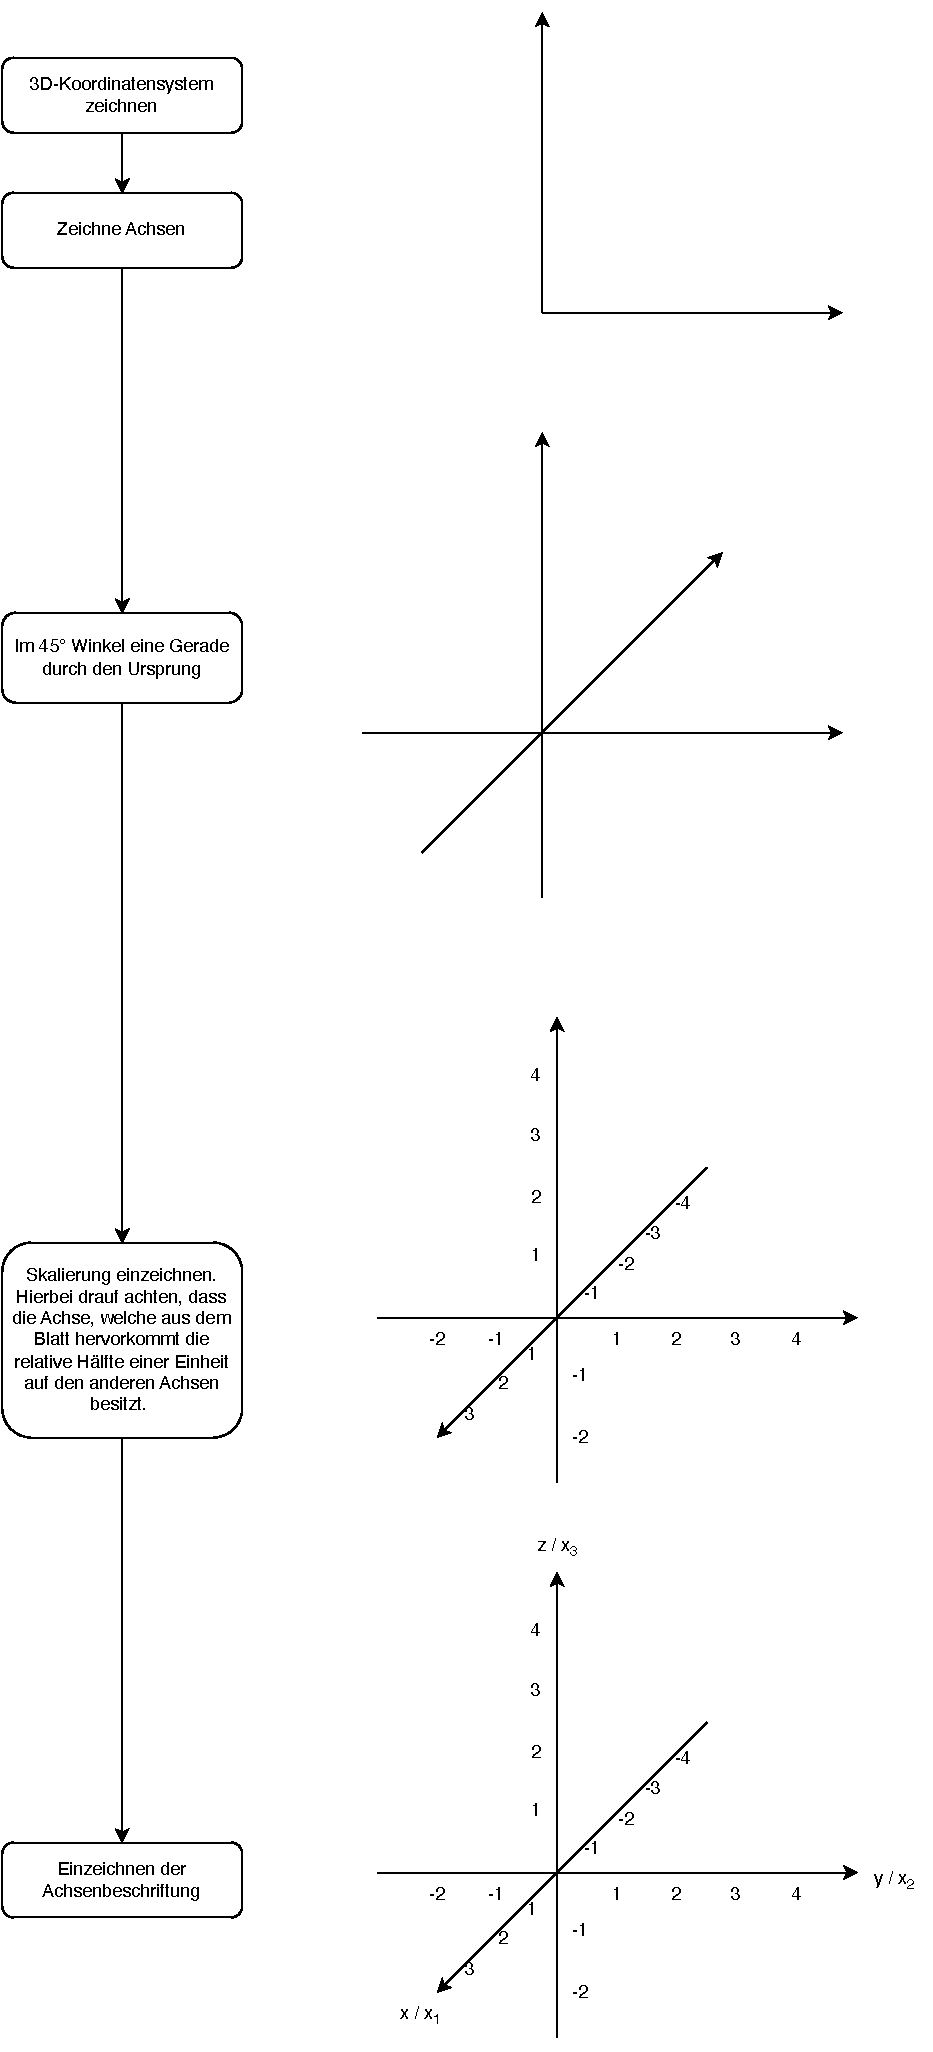
\includegraphics[width=9cm]{Algorithmen/karthesisches-Koordinatensystem-zeichen/karthesisches-Koordinatensystem-zeichen.drawio.pdf}
\subsection{Der dreidimensionale Raum}
Der dreidimensonale Raum wird beschrieben durch die 3 Achsen, die somit einem Punkt ermöglichen jede erdenkliche Position im Raum anzugeben. 


\subsection{Punkte einzeichnen}
Um einen Punkt in ein dreidimensonales Koordinatesystem einzuzeichen geht man wie folgt vor.
\begin{itemize}
	\item[1] Zuerst geht man die gegeben $x_1$-Koordinate entlang
	\item[2] Nun geht man die jeweiligen Schritte auf der $x_2$-Achse
	\item[3] Abschließend geht man nun relative Einheiten auf der $x_3$-Achse  
\end{itemize} 

\subsection{Punkt bestimmen}
Um einen Punkt im Koordinatensystem zu bestimmen wird mindestens eine Koordinate benötigt, da sonst eine unendlich große Zahle an Möglichkeiten entstehet. Ist eine Koordinate bekannt, eines eingezeichneten Punktes, kann man sich Hilfslinien einzeichnen, die paralell zu den Koordinateneben verlaufen. 

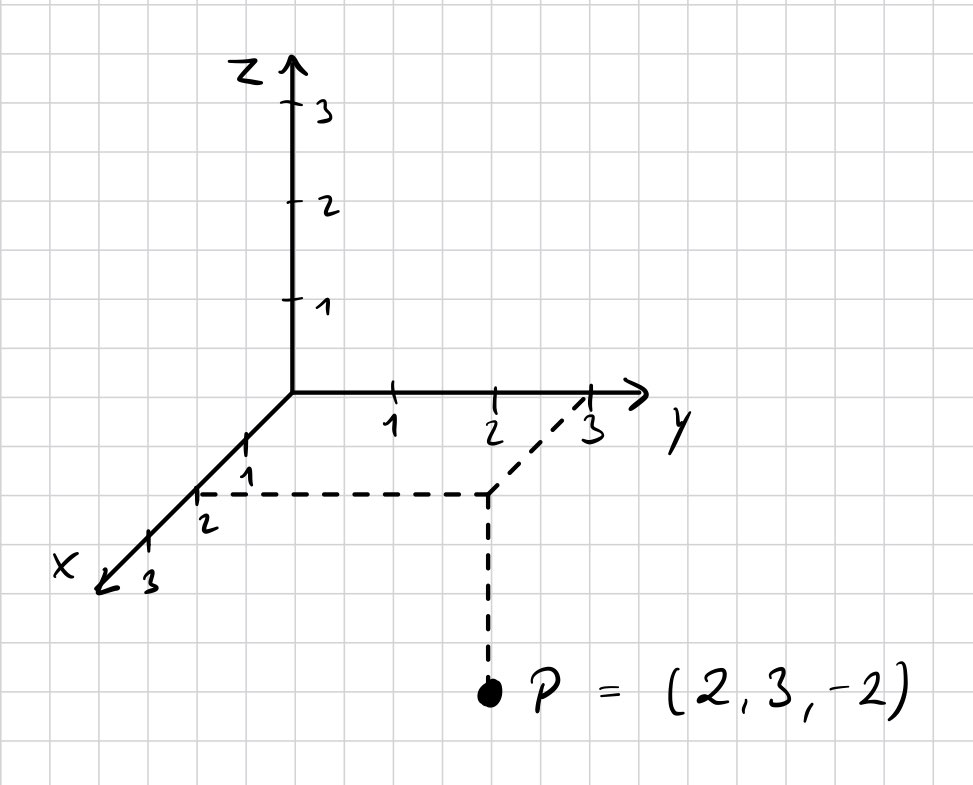
\includegraphics[width=10cm]{Media/punktablesen3dKoordinatensystem.jpg}